\documentclass[french, 11pt]{article}
\usepackage[utf8]{inputenc}
\usepackage[T1]{fontenc}
\usepackage{lmodern}
\usepackage{babel}
\usepackage{csquotes}
\pagestyle{empty}
\usepackage{soul}
\usepackage{setspace}
\usepackage{epigraph}
\usepackage{microtype}
\usepackage{xurl}
\usepackage{adjustbox}
\usepackage{float}


\sethlcolor{yellow}
\newcommand{\hlA}[1]{\begingroup\sethlcolor{yellow}\hl{#1}\endgroup}
\newcommand{\hlB}[1]{\begingroup\sethlcolor{cyan}\hl{#1}\endgroup}
\newcommand{\hlC}[1]{\begingroup\sethlcolor{pink}\hl{#1}\endgroup}

% --- Mathématiques ---
\usepackage{amsmath, amssymb, stmaryrd}

% --- TikZ ---
\usepackage{tikz}
\usetikzlibrary{calc, positioning, arrows.meta, shapes.geometric, shadows, decorations.pathreplacing, fit, backgrounds, matrix}

\definecolor{mycyan}{RGB}{0, 200, 255}
\definecolor{mygreen}{RGB}{0, 160, 50}
\definecolor{myorange}{RGB}{255, 120, 0}
\definecolor{myred}{RGB}{255, 0, 0}
\definecolor{mygrey}{RGB}{100, 100, 100}
\definecolor{bleufonce}{RGB}{30, 60, 110}

% --- Mise en page ---
\usepackage{geometry}
\usepackage{xcolor}
\usepackage{array, booktabs}
\usepackage{enumitem}

% --- Bibliographie ---
\usepackage[backend=biber, maxcitenames=2, style=authoryear]{biblatex}
\addbibresource{references.bib}
\renewcommand{\mkbibnamefamily}[1]{\textsc{#1}}
\renewcommand{\mkbibnameprefix}[1]{\textsc{#1}}

% --- Liens ---
\definecolor{bleufonce}{RGB}{0, 0, 130}
\usepackage[colorlinks=true, citecolor=bleufonce, linkcolor=bleufonce, urlcolor=bleufonce]{hyperref}
\begin{document}


\section*{De CamemBERT-base à \textsc{Emotyc}}
\label{sec:finetuning}

\noindent\textsc{Emotyc} est un modèle transformers conçu par \textcite{etienne2024} qui vise à détecter les catégories émotionnelles et les modes d'expression (cf. section précédente). Il s'agit d'une version affinée de CamemBERT-base \parencite{martin2020camembert}. La figure ci-dessous offre une vue synthétique de l'architecture d'\textsc{Emotyc} :


\begin{figure}[H]
\centering
\begin{adjustbox}{max totalheight=0.70\textheight, keepaspectratio}
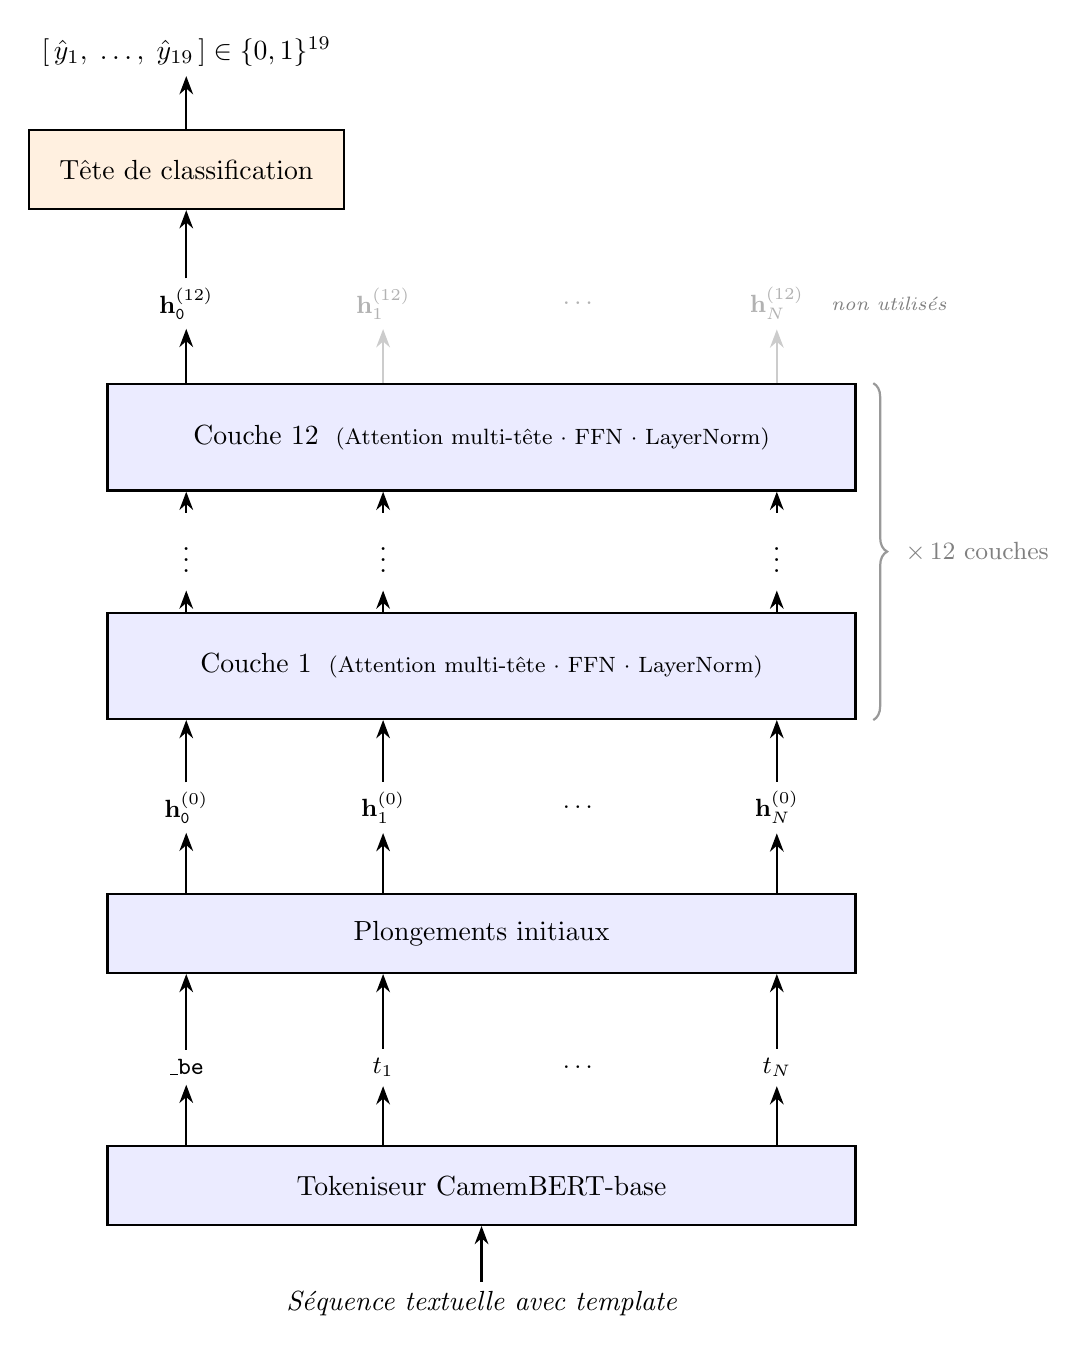
\begin{tikzpicture}[
    >=Stealth,
    inherited/.style={draw, thick, minimum width=9.5cm, minimum height=1cm,
                      align=center, fill=blue!8},
    added/.style={draw, thick, minimum width=4cm, minimum height=1cm,
                  align=center, fill=orange!12},
    lbox/.style={inherited, minimum height=1.35cm},
    rep/.style={font=\small},
    arr/.style={->, thick},
    garr/.style={->, thick, draw=black!20},
    ann/.style={font=\scriptsize\itshape, text=black!50}
]

\def\xs{0}
\def\xone{2.5}
\def\xdots{5.0}
\def\xn{7.5}
\def\xmid{3.75}

\node[font=\itshape] (input) at (\xmid, 0) {Séquence textuelle avec template};

\node[inherited] (tok) at (\xmid, 1.5) {Tokeniseur CamemBERT-base};
\draw[arr] (input) -- (tok);

\node[rep] (ts) at (\xs, 3) {\texttt{\_be}};
\node[rep] (t1) at (\xone, 3) {$t_1$};
\node[rep] (td) at (\xdots, 3) {$\dots$};
\node[rep] (tn) at (\xn, 3) {$t_N$};
\draw[arr] (tok.north -| ts) -- (ts);
\draw[arr] (tok.north -| t1) -- (t1);
\draw[arr] (tok.north -| tn) -- (tn);

\node[inherited] (emb) at (\xmid, 4.7)
  {Plongements initiaux};
\draw[arr] (ts) -- (ts |- emb.south);
\draw[arr] (t1) -- (t1 |- emb.south);
\draw[arr] (tn) -- (tn |- emb.south);

\node[rep] (h0s) at (\xs, 6.3) {$\mathbf{h}_{\texttt{0}}^{(0)}$};
\node[rep] (h01) at (\xone, 6.3) {$\mathbf{h}_1^{(0)}$};
\node[rep] (h0d) at (\xdots, 6.3) {$\dots$};
\node[rep] (h0n) at (\xn, 6.3) {$\mathbf{h}_N^{(0)}$};
\draw[arr] (emb.north -| h0s) -- (h0s);
\draw[arr] (emb.north -| h01) -- (h01);
\draw[arr] (emb.north -| h0n) -- (h0n);

\node[lbox] (L1) at (\xmid, 8.1)
  {Couche 1 \;{\footnotesize (Attention multi-tête $\cdot$ FFN $\cdot$ LayerNorm)}};
\draw[arr] (h0s) -- (h0s |- L1.south);
\draw[arr] (h01) -- (h01 |- L1.south);
\draw[arr] (h0n) -- (h0n |- L1.south);

\node (vds) at (\xs, 9.55) {$\vdots$};
\node (vd1) at (\xone, 9.55) {$\vdots$};
\node (vdn) at (\xn, 9.55) {$\vdots$};
\draw[arr] (L1.north -| vds) -- ([yshift=-3pt]vds.south);
\draw[arr] (L1.north -| vd1) -- ([yshift=-3pt]vd1.south);
\draw[arr] (L1.north -| vdn) -- ([yshift=-3pt]vdn.south);

\node[lbox] (L12) at (\xmid, 11.0)
  {Couche 12 \;{\footnotesize (Attention multi-tête $\cdot$ FFN $\cdot$ LayerNorm)}};
\draw[arr] ([yshift=3pt]vds.north) -- (vds |- L12.south);
\draw[arr] ([yshift=3pt]vd1.north) -- (vd1 |- L12.south);
\draw[arr] ([yshift=3pt]vdn.north) -- (vdn |- L12.south);

\draw[decorate,
      decoration={brace, amplitude=5pt, mirror, raise=4pt},
      thick, black!40]
  ([xshift=2pt]L1.south east) -- ([xshift=2pt]L12.north east)
  node[midway, right=12pt, font=\small, text=black!50]
    {$\times\,12$ couches};

\node[rep] (h12s) at (\xs, 12.7) {$\mathbf{h}_{\texttt{0}}^{(12)}$};
\node[rep, text=black!30] (h121) at (\xone, 12.7) {$\mathbf{h}_1^{(12)}$};
\node[rep, text=black!30] (h12d) at (\xdots, 12.7) {$\dots$};
\node[rep, text=black!30] (h12n) at (\xn, 12.7) {$\mathbf{h}_N^{(12)}$};
\draw[arr]  (L12.north -| h12s) -- (h12s);
\draw[garr] (L12.north -| h121) -- (h121);
\draw[garr] (L12.north -| h12n) -- (h12n);

\node[ann, right=0.1cm of h12n.east] {non utilisés};

\node[added] (head) at (\xs, 14.4) {Tête de classification};
\draw[arr] (h12s) -- (head);

\node[rep, font=\normalsize] (output) at (\xs, 15.9)
  {$[\,\hat{y}_1,\;\dots,\;\hat{y}_{19}\,] \in \{0,1\}^{19}$};
\draw[arr] (head) -- (output);

\end{tikzpicture}
\end{adjustbox}

\caption{Architecture d'\textsc{Emotyc}. Les modules en gris correspondent à la structure RoBERTa. Les paramètres / poids de ces modules ont  été mis à jour lors du fine-tuning. Le bloc orange est la tête de classification et a été ajoutée. Seul le vecteur $\mathbf{h}_{\texttt{0}}^{(12)}$ est transmis à la tête.}
\label{fig:archi-finetuning}
\end{figure}

\subsection*{Format d'entrée et rôle du token en position~0}
\label{subsec:format-entree}

\textcite{etienne2024} ont désactivé l'ajout des tokens spéciaux lors du fine-tuning\footnote{avec le paramètre $\texttt{add\_special\_tokens=False}$}, et n'ont pas ajouté le token \texttt{<s>} comme tout premier token. Ce réglage est important car c'est lui qui détermine l'argument donné en entrée à la tête de classification. En effet, les auteurs ont utilisé la librairie \texttt{transformers}\footnote{\url{https://github.com/huggingface/transformers/blob/main/src/transformers/models/roberta/modeling_roberta.py}}, qui implémente une tête de classification qui prend \textit{toujours} comme argument le vecteur à l'index~0 de la dernière couche cachée. Conventionnellement, ce vecteur est le token spécial \texttt{<s>}\footnote{Ceci s'explique en partie par le fait que, lors du pré-entraînement des modèles RoBERTa, les séquences d'entrée sont encadrées avec \texttt{<s>} et \texttt{</s>}.}, ce qui n'était jamais le cas dans le présent \textit{fine-tuning}. En désactivant l'ajout du token spécial \texttt{<s>} au début de la séquence, c'est simplement le \textit{tout premier token de la séquence donnée en entrée}, qui est utilisé pour la classification. Pour savoir quel est ce token, on peut se référer au fait que, dans le fine-tuning d'\textsc{Emotyc}, les entrées avaient invariablement le format :
\begin{center}
\texttt{before:\{previous\}</s>current:\{target\}</s>after:\{next\}</s>}
\end{center}
où \texttt{{previous}}, \texttt{{target}} et \texttt{{next}} désignent respectivement la phrase précédente, la phrase cible (à classifier) et la phrase suivante (\cite[p.\,5]{etienne2024}). Le tout premier mot \og \texttt{before} \fg est segmenté par le tokeniseur en trois sous-mots :

$$\text{Tokeniser.tokenise}(\texttt{"before"}) = \bigl[\texttt{be},\, \texttt{for},\, \texttt{e}\bigr]$$

Ainsi, le token en position~0 est \og \texttt{be}  \fg  \footnote{Il s'agit plus précisément de \og\,\texttt{\_be}\,\fg{} car \texttt{CamembertTokenizer} ajoute en préfixe le caractère \og\,\texttt{\_}\,\fg{} lorsqu'il y a un espace avant le mot.}. L'embedding associé à ce token qui sort de la toute dernière couche est noté ci-dessus par $\mathbf{h}_{\texttt{0}}^{(12)}$ et c'est ce qui sert pour la classification. Dans la mesure où il s'agit d'un fragment lexical courant et présent dans de nombreux contextes, il est probable que le fine-tuning ait adapté certains paramètres (par exemple les matrices d'attention) pour que ce \og \texttt{be} \fg{} joue le rôle d'agrégateur des signaux sémantiques pertinents pour la classification.

Il est intéressant de noter que, dans nos tests, même si les meilleures performances (en inférence) du modèle \textsc{emotyc} sont sur des entrées avec le template et en désactivant l'ajout des tokens spéciaux, les performances avec le template mais en activant les tokens spéciaux sont très bonnes et proches du premier cas. Cela suggère que, dans les deux cas, l'architecture Transformer parvient à diriger l'information pertinente vers la position~0 (vers le token associé à \texttt{<s>} ou vers celui associé à \texttt{be}).


Le fine-tuning de CamemBERT-base a été réalisé suivant une stratégie en deux temps, visant à stabiliser l'apprentissage sur des classes fortement déséquilibrées\footnote{Les détails donnés par \textcite[p.5]{etienne2024} sont : "The optimizer is Adam with a learning rate of $10^{-5}$ (no decay) and batches of 8 examples (...) Notably, a weighting between classes is adopted so as not to overly favor the majority classes. The maximum weighting factor is capped at 50 to, conversely, not give too much importance to very rare classes."}. Les deux phases relatées par \textcite{etienne2024} sont les suivantes : Premièrement, un premier affinage effectué uniquement sur la tâche de détection de la présence ou absence d'émotion. La couche de classification comporte alors une seule sortie dans \{0,1\}. Deuxièmement, un fine-tuning multi-tâches et à granularité plus fine, où le modèle issu de la première phase est  affiné sur les 4~tâches simultanément (détection d'émotion, modes, types, catégories).


\end{document}
